% Questao 2 - texto, analise, figuras e trechos de codigo
%
% No preambulo do Overleaf, usar:
% \usepackage{graphicx}
% \usepackage{float}
% \usepackage{xcolor}
% \usepackage{listings}
%
% Sugestao de configuracao para os codigos:
% \lstset{
%   language=Java,
%   basicstyle=\ttfamily\footnotesize,
%   keywordstyle=\color{blue},
%   commentstyle=\color{gray},
%   stringstyle=\color{teal},
%   breaklines=true,
%   frame=single,
%   showstringspaces=false,
%   columns=fullflexible
% }

\lstset{
  language=Java,
  basicstyle=\ttfamily\footnotesize,
  keywordstyle=\color{blue},
  commentstyle=\color{gray},
  stringstyle=\color{teal},
  breaklines=true,
  frame=single,
  showstringspaces=false,
  columns=fullflexible
}

\subsection{Questao 2 - Clinica Veterinaria em Tempo Real}

Na segunda questao foi desenvolvida uma simulacao de uma clinica veterinaria em funcionamento. A ideia foi representar um ambiente em que varias atividades podem acontecer ao mesmo tempo: chegada de animais, cadastro na recepcao, atendimento veterinario, vacinacao, banho e tosa, exames laboratoriais e casos de emergencia.

Para deixar a simulacao mais proxima de um sistema real, cada atendimento possui dados do pet e do tutor. Foram incluidos nome do animal, especie, raca, sexo, nome do tutor, telefone, bairro, servico solicitado, ocorrencia do atendimento, funcionario responsavel e valor simulado do servico. Esses dados tambem aparecem na interface grafica e no historico final.

\subsubsection{Versao sequencial}

A versao sequencial representa a clinica sem uso de threads. Nesse caso, existe apenas um fluxo de execucao: um animal chega, passa pela recepcao, recebe atendimento e somente depois o proximo animal inicia o processo. Na pratica, essa versao funciona como se houvesse um unico funcionario responsavel por todos os atendimentos.

O trecho principal da versao sequencial esta no Codigo~\ref{cod:q2-sequencial}. O laco percorre a quantidade de animais definida pelo usuario e executa as etapas sempre na mesma ordem.

\begin{lstlisting}[caption={Fluxo principal da versao sequencial.}, label={cod:q2-sequencial}]
long inicio = System.nanoTime();
for (int i = 1; i <= quantidadeAnimais; i++) {
    AtendimentoVeterinario atendimento = AtendimentoVeterinario.novo(i);
    simularChegada(atendimento, intervaloChegadaMs);
    recepcionar(atendimento);
    atender(atendimento);
}
long fim = System.nanoTime();

double tempoTotalMs = (fim - inicio) / 1_000_000.0;
\end{lstlisting}

Mesmo quando aparece uma emergencia, ela so e tratada quando chega sua vez no fluxo. Isso mostra a limitacao da programacao sequencial tradicional para esse tipo de problema: nao ha paralelismo entre recepcao e atendimento.

\subsubsection{Versao com threads}

Na versao com threads, a clinica passa a ter uma thread para a recepcao e varias threads para os funcionarios. A recepcao cadastra os animais e coloca cada atendimento em uma fila compartilhada. Os funcionarios retiram atendimentos dessa fila e executam os servicos em paralelo.

Foram usados dois recursos importantes da biblioteca Java. O primeiro foi \texttt{PriorityBlockingQueue}, que permite uma fila segura para acesso concorrente e ainda respeita prioridades. O segundo foi \texttt{AtomicInteger}, usado para contar os atendimentos concluidos sem conflito entre as threads.

\begin{lstlisting}[caption={Criacao da fila compartilhada, contador e threads de funcionarios.}, label={cod:q2-threads-main}]
PriorityBlockingQueue<AtendimentoVeterinario> fila =
        new PriorityBlockingQueue<AtendimentoVeterinario>();
AtomicInteger atendimentosConcluidos = new AtomicInteger(0);
Funcionario[] funcionarios = new Funcionario[quantidadeFuncionarios];

Recepcao recepcao = new Recepcao(
        fila,
        quantidadeAnimais,
        intervaloChegadaMs,
        quantidadeFuncionarios);
recepcao.start();

for (int i = 0; i < quantidadeFuncionarios; i++) {
    funcionarios[i] = new Funcionario(i + 1, fila, atendimentosConcluidos);
    funcionarios[i].start();
}
\end{lstlisting}

A prioridade das emergencias foi definida na propria classe \texttt{AtendimentoVeterinario}. Quando dois atendimentos sao comparados, os casos de emergencia ficam antes dos atendimentos normais. Se ambos tiverem a mesma prioridade, a ordem de chegada e mantida.

\begin{lstlisting}[caption={Criterio de prioridade dos atendimentos.}, label={cod:q2-prioridade}]
@Override
public int compareTo(AtendimentoVeterinario outro) {
    if (this.fimExpediente && outro.fimExpediente) {
        return 0;
    }
    if (this.fimExpediente) {
        return 1;
    }
    if (outro.fimExpediente) {
        return -1;
    }
    if (this.emergencia != outro.emergencia) {
        return this.emergencia ? -1 : 1;
    }
    return Long.compare(this.ordemChegada, outro.ordemChegada);
}
\end{lstlisting}

Cada funcionario fica em execucao ate receber um marcador de fim de expediente. Enquanto isso, ele retira atendimentos da fila, registra o inicio do servico, espera o tempo simulado do procedimento e incrementa o contador de atendimentos concluidos.

\begin{lstlisting}[caption={Execucao de uma thread de funcionario.}, label={cod:q2-funcionario}]
while (true) {
    AtendimentoVeterinario atendimento = fila.take();
    if (atendimento.fimExpediente) {
        log(getName() + " recebeu fim de expediente.");
        break;
    }

    log(getName() + " INICIOU " + atendimento.servico
            + " para " + atendimento.descricaoCompleta());

    if (atendimento.emergencia) {
        log(getName() + " priorizou emergencia.");
    }

    Thread.sleep(atendimento.duracaoMs);
    int total = atendimentosConcluidos.incrementAndGet();
    log(getName() + " FINALIZOU " + atendimento.nomePet
            + ". Total concluido: " + total);
}
\end{lstlisting}

\subsubsection{Interface grafica}

Tambem foi criada uma interface grafica em Java Swing para acompanhar a simulacao de forma visual. A tela permite configurar a quantidade de funcionarios, a quantidade de animais e o intervalo de chegada. Durante a execucao, a interface mostra a fila, os funcionarios em atendimento, o historico, os logs, a receita simulada, o tempo total e o progresso geral.

Na interface, os dados dos atendimentos aparecem em tabelas. O nome do pet recebe cor diferente conforme o sexo, sendo rosa para femeas e azul para machos. A tela tambem diferencia os animais por especie e raca, possui uma logo propria da clinica e permite salvar o historico em CSV ou em relatorio TXT.

\begin{figure}[H]
    \centering
    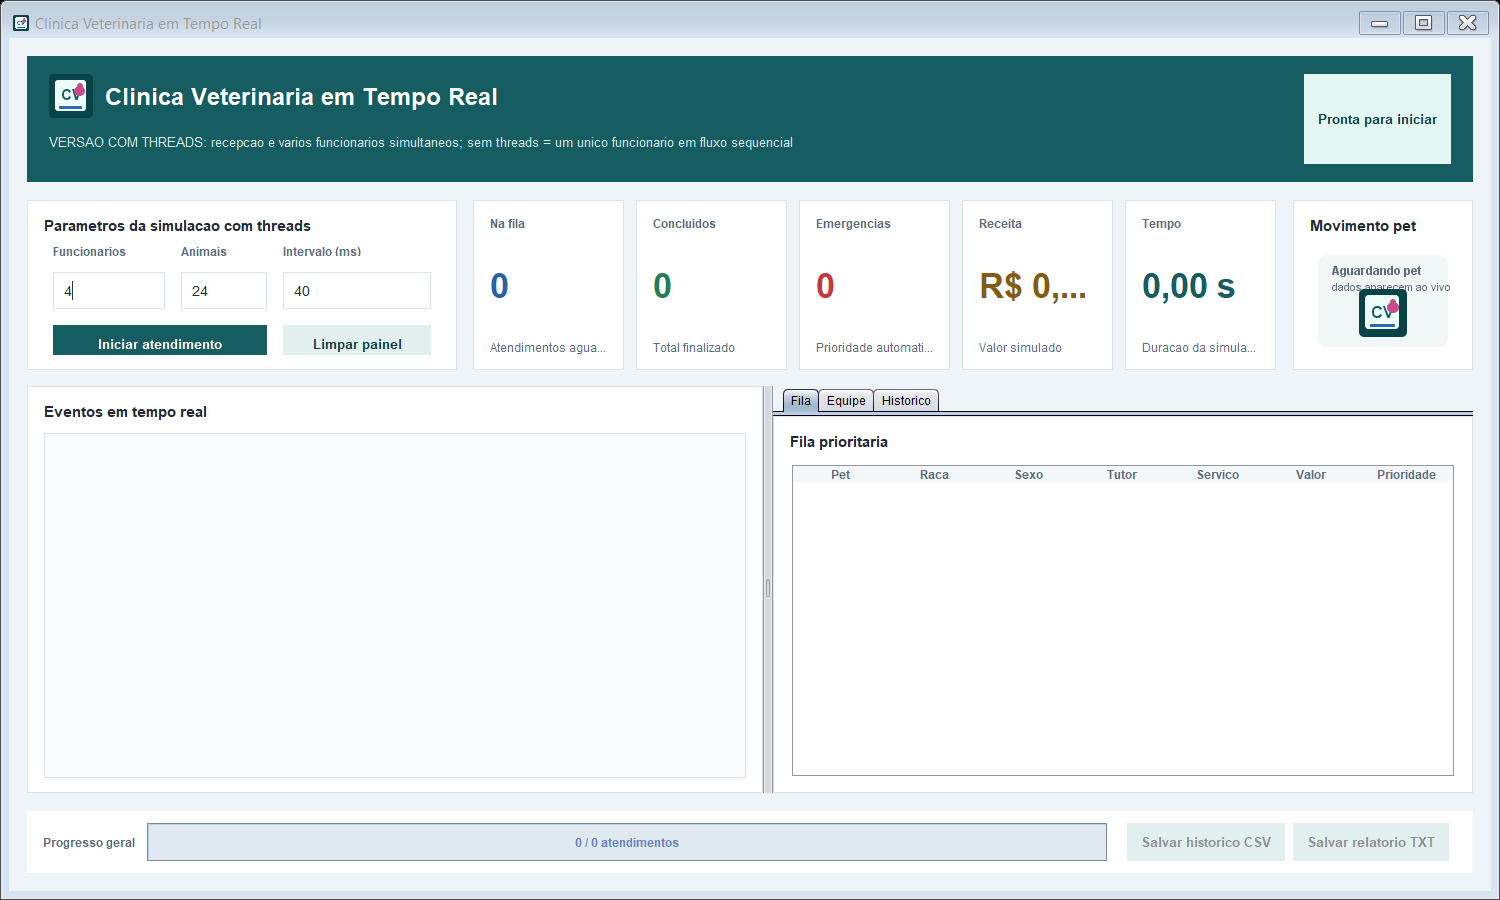
\includegraphics[width=\textwidth]{imagens/q2_interface_inicial.png}
    \caption{Tela inicial da clinica veterinaria, com os campos para configurar funcionarios, quantidade de animais e intervalo de chegada.}
    \label{fig:q2-interface-inicial}
\end{figure}

\begin{figure}[H]
    \centering
    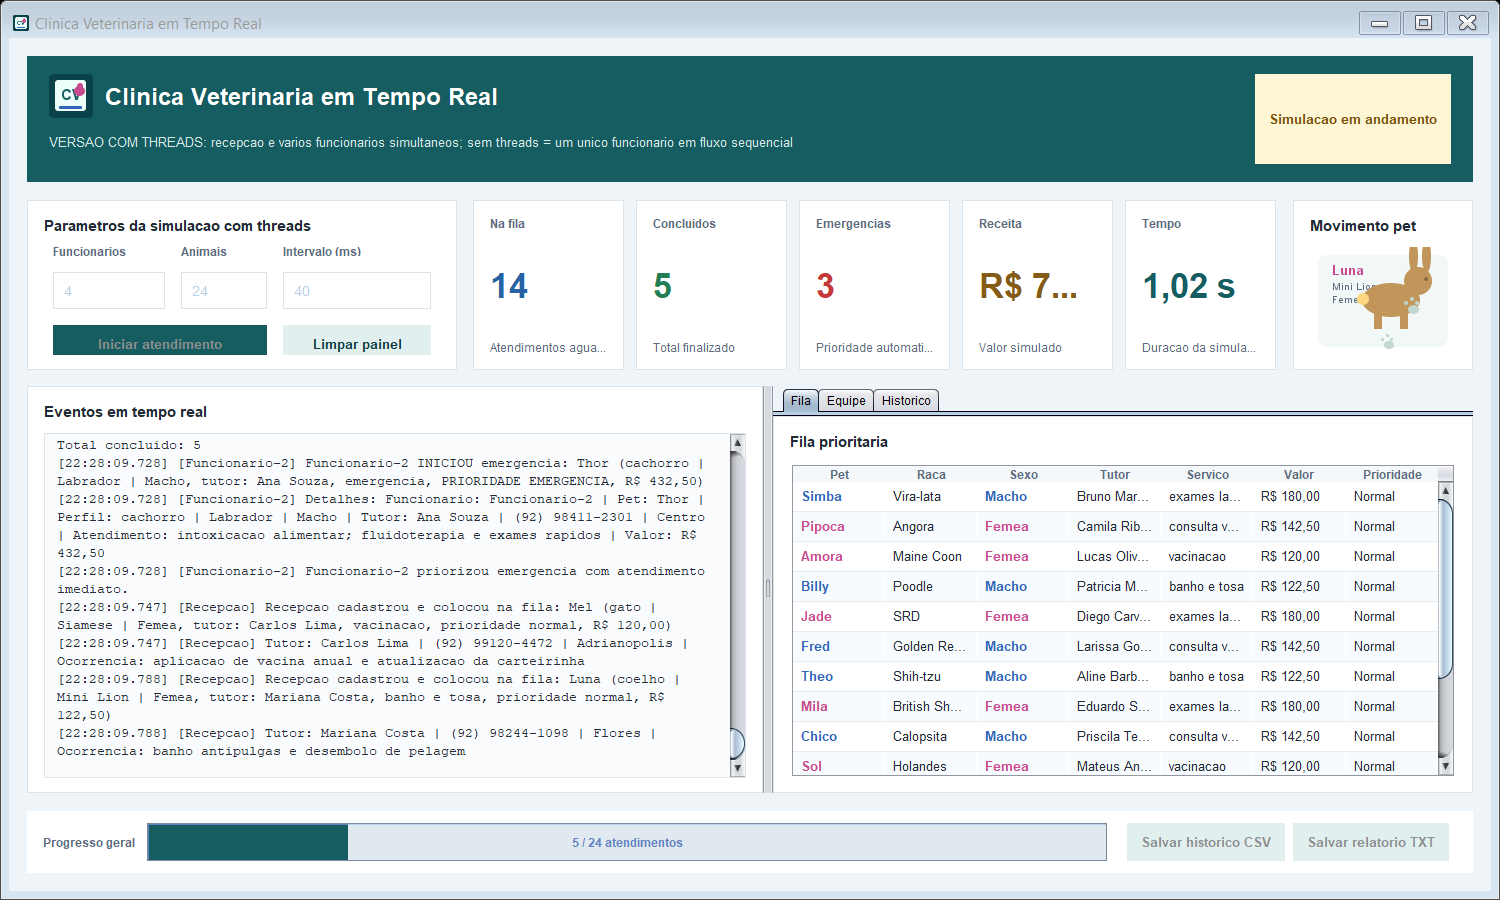
\includegraphics[width=\textwidth]{imagens/q2_interface_execucao_fila.png}
    \caption{Simulacao em execucao na aba da fila prioritaria. A tela mostra atendimentos aguardando, logs em tempo real e emergencia sendo priorizada por uma thread de funcionario.}
    \label{fig:q2-interface-execucao-fila}
\end{figure}

\begin{figure}[H]
    \centering
    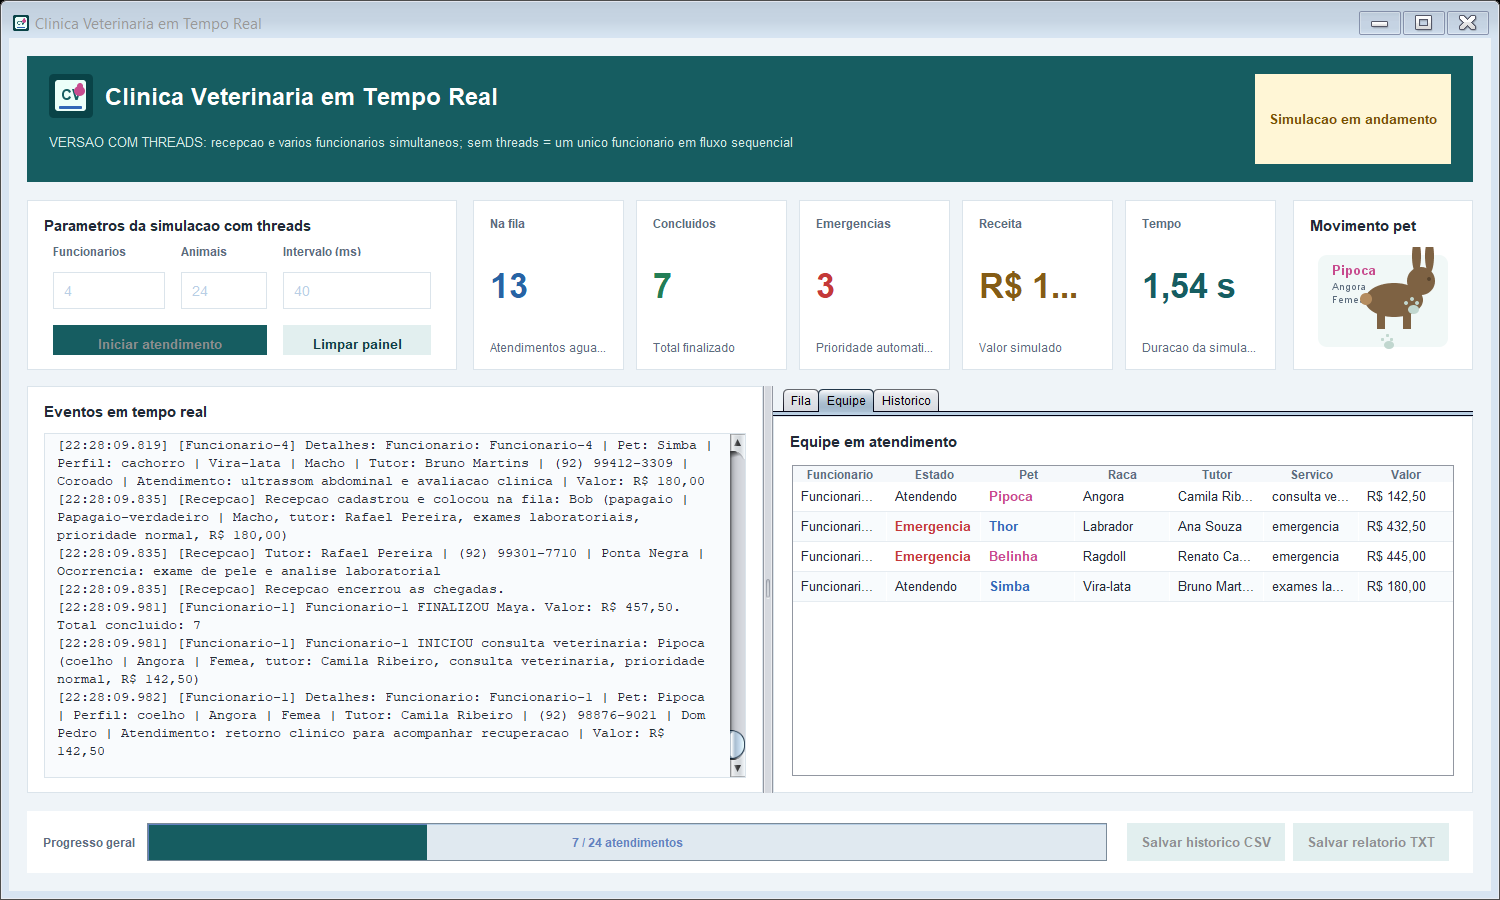
\includegraphics[width=\textwidth]{imagens/q2_interface_execucao_equipe.png}
    \caption{Aba da equipe durante a execucao. Cada linha representa um funcionario em uma thread separada, permitindo observar atendimentos simultaneos e casos emergenciais.}
    \label{fig:q2-interface-execucao-equipe}
\end{figure}

\begin{figure}[H]
    \centering
    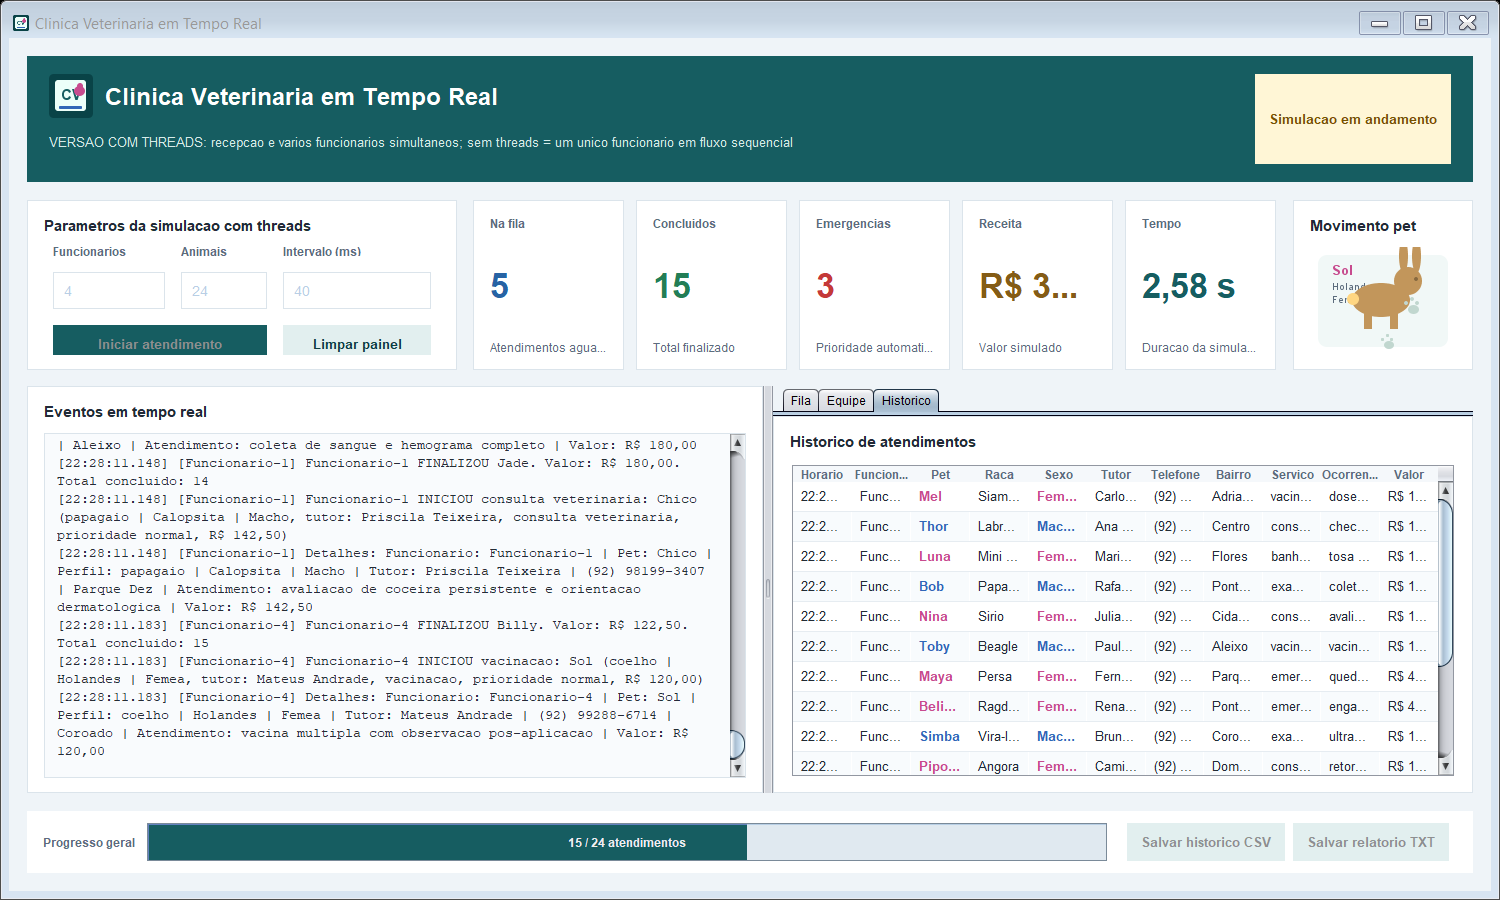
\includegraphics[width=\textwidth]{imagens/q2_interface_historico_parcial.png}
    \caption{Historico parcial durante a simulacao, registrando os atendimentos que ja foram finalizados enquanto outros continuam em execucao.}
    \label{fig:q2-interface-historico-parcial}
\end{figure}

\begin{figure}[H]
    \centering
    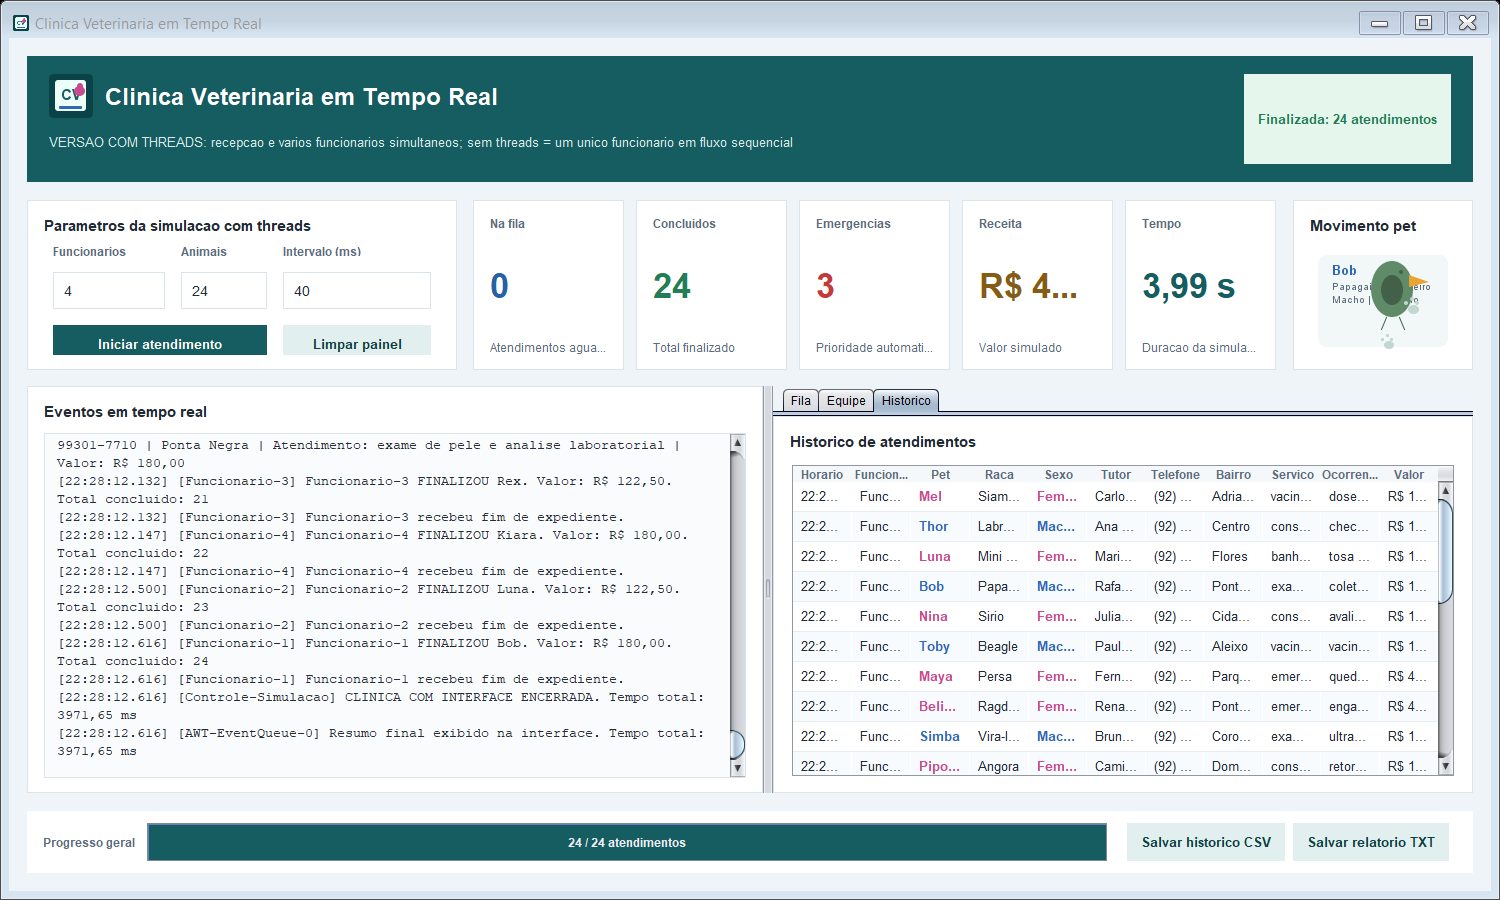
\includegraphics[width=\textwidth]{imagens/q2_interface_final_historico.png}
    \caption{Tela final com o historico dos atendimentos, incluindo pet, tutor, funcionario, servico, ocorrencia e valor simulado.}
    \label{fig:q2-interface-final-historico}
\end{figure}

\begin{figure}[H]
    \centering
    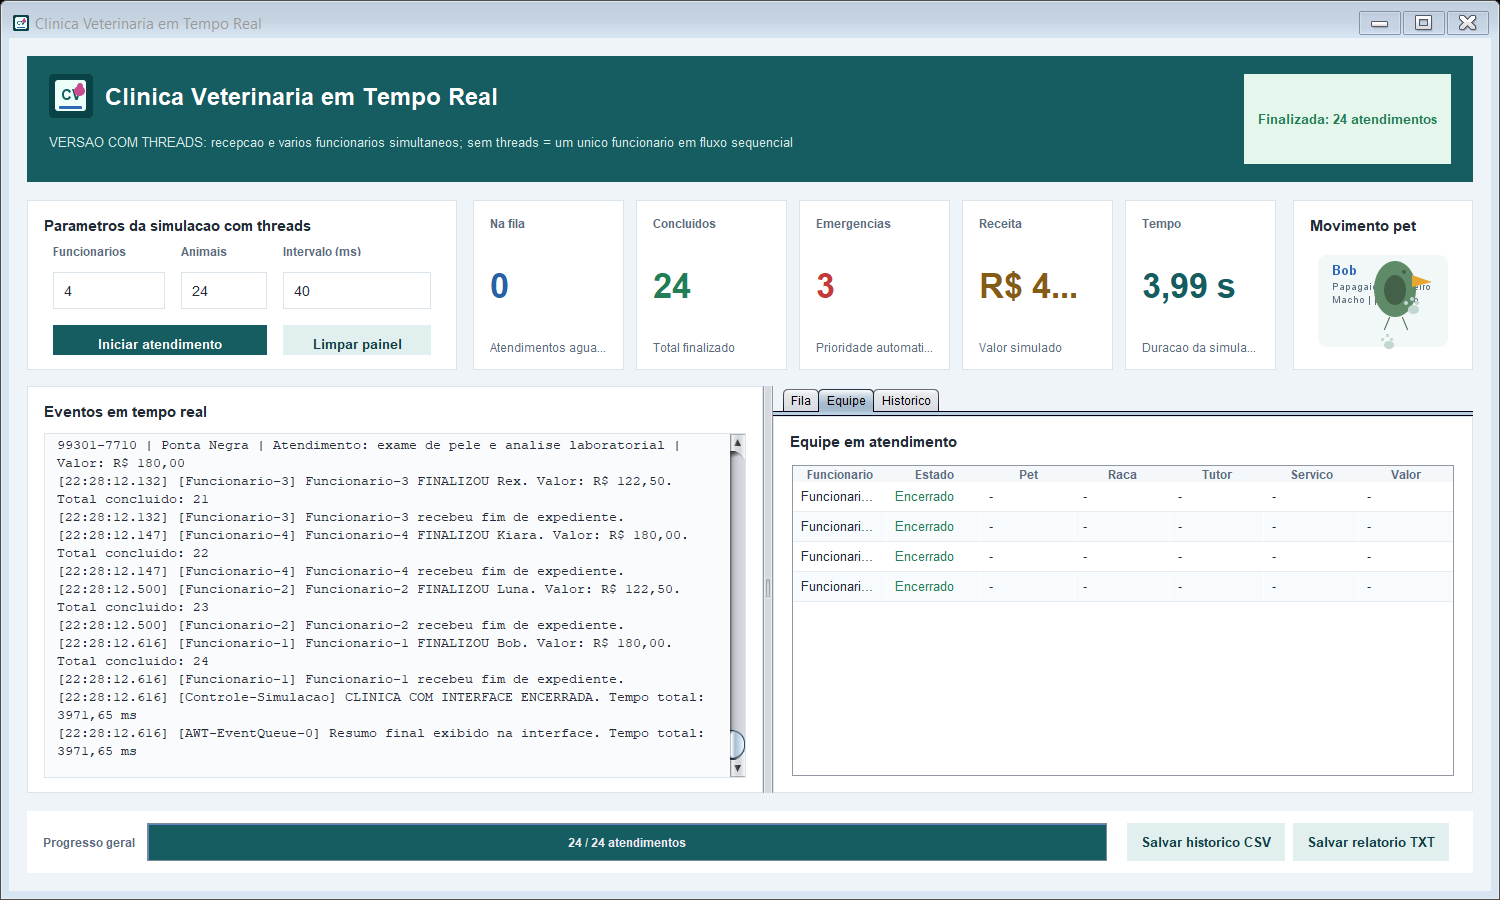
\includegraphics[width=\textwidth]{imagens/q2_interface_final_equipe.png}
    \caption{Tela final na aba da equipe, mostrando todos os funcionarios encerrados, progresso completo e botoes habilitados para salvar historico ou relatorio.}
    \label{fig:q2-interface-final-equipe}
\end{figure}

\subsubsection{Analise dos resultados}

Para comparar as duas versoes, foi executado um teste com a mesma carga: 12 animais e intervalo de chegada de 40 ms. Na versao com threads foram usados 4 funcionarios. Os tempos obtidos estao na Tabela~\ref{tab:q2-comparacao}.

\begin{table}[H]
    \centering
    \caption{Comparacao entre a versao sequencial e a versao com threads.}
    \label{tab:q2-comparacao}
    \resizebox{\textwidth}{!}{%
    \begin{tabular}{lcccc}
        \hline
        Modo & Funcionarios/threads & Animais & Intervalo (ms) & Tempo (ms) \\
        \hline
        Sequencial & 1 & 12 & 40 & 8358,26 \\
        Com threads & 4 & 12 & 40 & 2134,33 \\
        \hline
    \end{tabular}
    }
\end{table}

Com esses valores, a versao com threads foi aproximadamente 3,92 vezes mais rapida:

\[
S = \frac{8358,26}{2134,33} \approx 3,92
\]

O resultado era esperado, porque os atendimentos simulados sao independentes entre si. Enquanto a versao sequencial fica presa a um unico atendimento por vez, a versao paralela distribui os servicos entre os funcionarios. Assim, recepcao e atendimento podem ocorrer de forma sobreposta, e varios pets podem estar em atendimento ao mesmo tempo.

Outro ponto observado foi o tratamento das emergencias. Na versao com threads, quando um atendimento emergencial entra na fila, ele passa a ter prioridade sobre os atendimentos normais que ainda nao foram iniciados. Isso torna a simulacao mais adequada ao tema escolhido, pois em uma clinica real casos urgentes nao devem seguir apenas a ordem simples de chegada.

Os tempos medidos nao representam a duracao real de uma consulta veterinaria, pois os procedimentos foram simulados com \texttt{Thread.sleep}. Ainda assim, eles servem para demonstrar o comportamento concorrente do sistema e a diferenca entre uma execucao sequencial e uma execucao com varias threads.

\subsubsection{Conclusao da Questao 2}

A versao sequencial cumpriu o papel de mostrar o funcionamento basico da clinica em um unico fluxo. Ja a versao com threads representou melhor a ideia de uma clinica em tempo real, com recepcao e funcionarios atuando simultaneamente. A fila prioritaria, o contador atomico e os logs com nome das threads ajudaram a deixar visivel o funcionamento da concorrencia.

Com a interface grafica, ficou mais facil acompanhar o estado da simulacao e registrar os atendimentos realizados. Dessa forma, a aplicacao demonstra tanto o ganho de desempenho quanto a organizacao de tarefas simultaneas, que e um dos principais objetivos do uso de threads em Sistemas Operacionais.
